\documentclass[runningheads]{llncs}

% ---------------------------------------------------------------
% Include basic ECCV package

% TODO REVIEW: Insert your submission number below by replacing '*****'
% TODO FINAL: Comment out the following line for the camera-ready version
\usepackage[review,year=2026,ID=*****]{eccv}
% TODO FINAL: Un-comment the following line for the camera-ready version
%\usepackage{eccv}

% ---------------------------------------------------------------
% Other packages

% Commonly used abbreviations (\eg, \ie, \etc, \cf, \etal, etc.)
\usepackage{eccvabbrv}

% Include other packages here, before hyperref.
\usepackage{graphicx}
\usepackage{booktabs}
\usepackage{amsmath}
\usepackage{amssymb}
\usepackage{algorithm}
\usepackage{algorithmic}
\usepackage{multirow}
\usepackage{subcaption}

% The "axessiblity" package can be found at: https://ctan.org/pkg/axessibility?lang=en
\usepackage[accsupp]{axessibility}  % Improves PDF readability for those with disabilities.


% ---------------------------------------------------------------
% Hyperref package

% TODO FINAL: Comment out the following line for the camera-ready version
%\usepackage[pagebackref,breaklinks,colorlinks,citecolor=eccvblue]{hyperref}
% TODO FINAL: Un-comment the following line for the camera-ready version
\usepackage{hyperref}

% Support for ORCID icon
\usepackage{orcidlink}

% Custom math operators
\DeclareMathOperator{\sigmoid}{sigmoid}
\newcommand{\bx}{\mathbf{x}}
\newcommand{\bc}{\mathbf{c}}
\newcommand{\bz}{\mathbf{z}}
\newcommand{\bm}{\mathbf{m}}
\newcommand{\btau}{\boldsymbol{\tau}}


\begin{document}

% ---------------------------------------------------------------
\title{Switch \& Stitch: Long-Horizon Hand-Object Motion Generation via Diffusion-Based Transition Scheduling}

\titlerunning{Switch \& Stitch: Long-Horizon Hand-Object Motion}

% TODO FINAL: Replace with your author list.
\author{First Author\inst{1} \and
Second Author\inst{1} \and
Third Author\inst{1}}

\authorrunning{F.~Author et al.}

% TODO FINAL: Replace with your institution list.
\institute{Institution, City, Country\\
\email{\{first,second,third\}@institution.edu}}

\maketitle


% ============================================================
% ABSTRACT
% ============================================================
\begin{abstract}
Generating long-horizon hand-object interaction sequences from multi-sentence natural language remains an open challenge.
Existing methods either produce single-sentence body motions or synthesize short hand-object grasps, but none address the composition of extended, physically plausible manipulation sequences.
We present \textbf{Switch~\&~Stitch}, a three-module framework that (i)~parses a multi-sentence paragraph into an ordered generation plan via a \emph{Text Orchestrator}, (ii)~synthesizes per-sentence motion segments using DiffH2O, a two-phase hand-object diffusion backbone, and (iii)~stitches consecutive segments through a novel \emph{Switch Scheduler}---a boundary-conditioned diffusion transformer that generates temporally coherent transitions.
The Switch Scheduler conditions on boundary frames from adjacent segments and concatenated CLIP text embeddings, producing smooth transitions via learned sigmoid-ramp blending.
We evaluate on the GRAB and OakInk2 benchmarks, demonstrating that our approach produces long, coherent manipulation sequences while maintaining physical plausibility at segment boundaries.
To our knowledge, this is the first framework for generating long-term hand-object motion from multi-sentence text.
\keywords{Hand-object interaction \and Motion generation \and Diffusion models \and Long-term synthesis \and Text-driven generation}
\end{abstract}


% ============================================================
% 1. INTRODUCTION
% ============================================================
\section{Introduction}
\label{sec:intro}

Consider a robotic assistant that must execute the instruction: \emph{``Pick up the mug, pour water into it, then place it on the table and wave goodbye.''}
Performing this task requires generating a temporally extended hand-object manipulation sequence in which each sub-action is physically plausible, the object state is tracked across transitions, and the overall motion flows naturally from one action to the next.
Such long-horizon, text-driven hand-object motion generation is essential for applications in robotics, virtual reality, character animation, and assistive technology, yet it remains largely unsolved.

Prior work on text-driven motion synthesis has made substantial progress on single-sentence generation for full-body motion.
Diffusion-based approaches such as MDM~\cite{tevet2023human}, MotionDiffuse~\cite{zhang2022motiondiffuse}, MLD~\cite{chen2023executing}, and T2M-GPT~\cite{zhang2023t2mgpt} generate diverse, high-quality body motions from short text prompts.
In the hand-object domain, DiffH2O~\cite{christen2024diffh2o} introduced a two-phase diffusion pipeline that synthesizes grasping and interaction motions conditioned on text and object geometry, while datasets such as GRAB~\cite{taheri2020grab} and OakInk2~\cite{zhan2024oakink2} provide rich annotations.
However, these methods are limited to \emph{single-action, fixed-length} outputs.
Separately, long-term body motion composition methods---TEACH~\cite{athanasiou2022teach}, DoubleTake~\cite{shafir2024doubletake}, FlowMDM~\cite{barquero2024seamless}, and PriorMDM~\cite{shafir2024priormdm}---chain multiple body motions but do not model hand-object physics.
A critical gap therefore exists at the intersection of these two lines of work: no existing method generates long-horizon hand-object interactions from multi-sentence text.

Bridging this gap introduces several technical challenges.
First, \textbf{transition coherence}: naively concatenating independently generated segments produces velocity and pose discontinuities at boundaries, leading to visual artifacts such as sudden jumps or interpenetration.
Second, \textbf{object state continuity}: the object pose at the end of one action must match the start of the next, which is not guaranteed by independent generation.
Third, \textbf{physical plausibility across time}: contact forces, hand-object signed distance fields (SDFs), and grasp stability must be maintained not only within segments but also through transitions.
Fourth, \textbf{natural language decomposition}: multi-sentence prompts must be parsed into an ordered sequence of actions with estimated durations and identified objects.

We address these challenges with \textbf{Switch~\&~Stitch}, a modular framework comprising three components (\cref{fig:pipeline}).
The \emph{Text Orchestrator} decomposes a multi-sentence prompt into individual sentences, extracts objects and temporal markers, and plans segment durations.
The \emph{Segment Generator} produces per-sentence motion using DiffH2O's two-phase diffusion backbone (\cref{fig:diffh2o}), which first generates a grasping motion and then synthesizes the full hand-object interaction with inpainting guidance.
The \emph{Switch Scheduler}---our core contribution---is a boundary-conditioned diffusion transformer that generates smooth transitions between consecutive segments.
It conditions on the last $k$ frames of one segment and the first $k$ frames of the next, along with concatenated CLIP embeddings of both sentences, and produces a denoised transition that is blended into the sequence with learned sigmoid-ramp weights.

Our contributions are:
\begin{enumerate}
    \item The first framework for generating long-term hand-object manipulation sequences from multi-sentence natural language descriptions.
    \item The \textbf{Switch Scheduler}, a boundary-conditioned diffusion transformer that generates physically plausible transitions between motion segments with learned blending.
    \item A \textbf{Text Orchestrator} that automatically decomposes multi-sentence prompts into structured generation plans with temporal reasoning, object extraction, and duration planning.
    \item Evaluation on the GRAB~\cite{taheri2020grab} and OakInk2~\cite{zhan2024oakink2} datasets demonstrating coherent long-horizon synthesis with maintained physical plausibility.
\end{enumerate}


% ============================================================
% FIGURE 1: Pipeline Overview
% ============================================================
\begin{figure}[t]
  \centering
  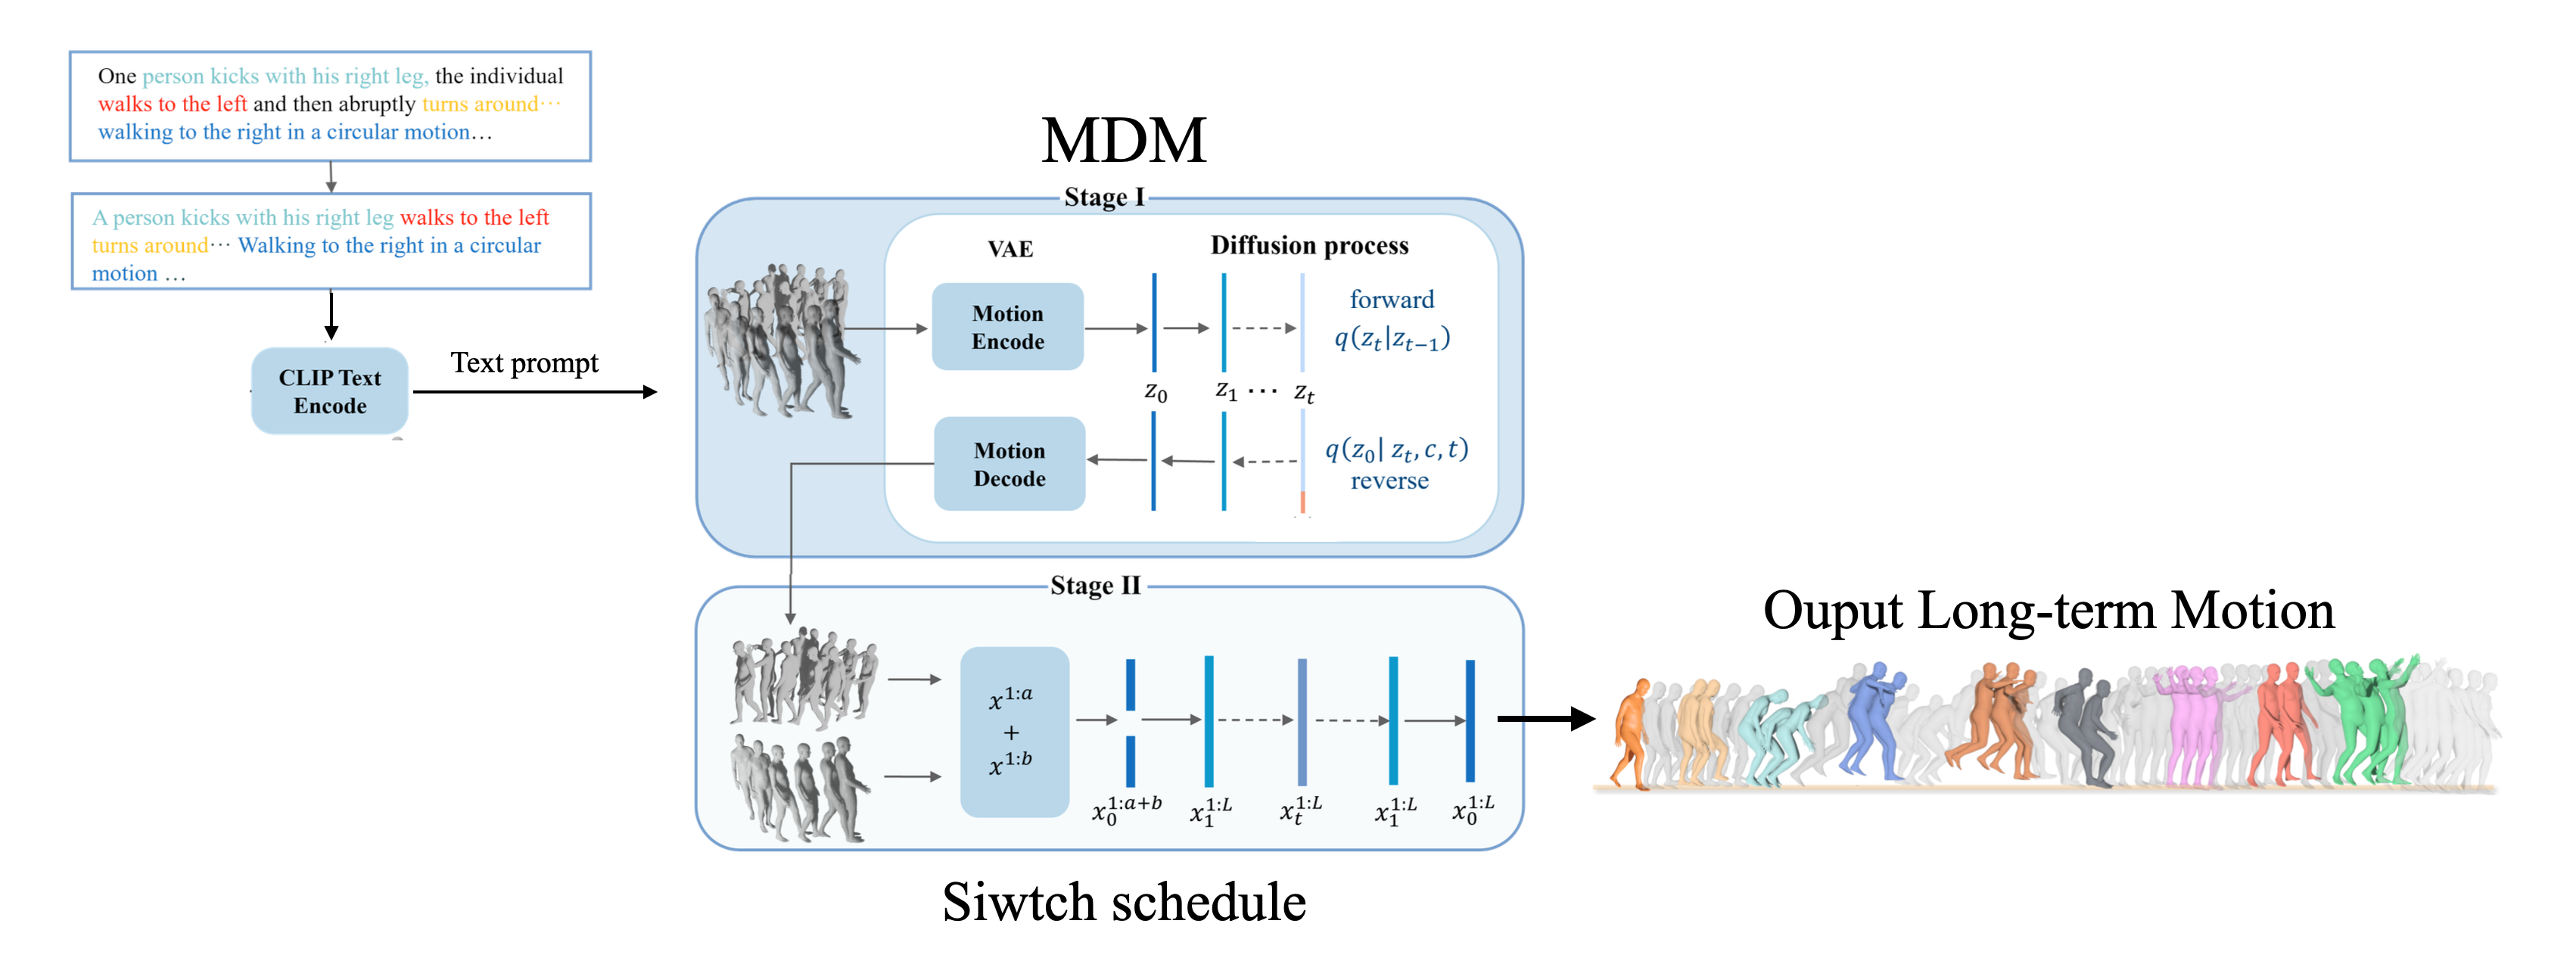
\includegraphics[width=\linewidth]{figure_1.png}
  \caption{\textbf{Overview of Switch~\&~Stitch.} Given a multi-sentence text prompt, the Text Orchestrator decomposes it into individual sentences with duration estimates. Stage~I: the Segment Generator (DiffH2O backbone) produces per-sentence hand-object motions. Stage~II: the Switch Scheduler generates smooth transitions between consecutive segments via boundary-conditioned diffusion, yielding a temporally coherent long-horizon sequence.}
  \label{fig:pipeline}
\end{figure}


% ============================================================
% 2. RELATED WORK
% ============================================================
\section{Related Work}
\label{sec:related}

\subsection{Text-Driven Motion Synthesis}
Text-conditioned human motion generation has advanced rapidly with diffusion models.
MDM~\cite{tevet2023human} applies a transformer-based denoiser directly in motion space with classifier-free guidance~\cite{ho2022classifier}.
MotionDiffuse~\cite{zhang2022motiondiffuse} introduces body-part-aware generation with fine-grained text control.
MLD~\cite{chen2023executing} performs diffusion in a learned latent space for faster sampling, while T2M-GPT~\cite{zhang2023t2mgpt} discretizes motion into tokens for autoregressive generation.
MotionCLIP~\cite{tevet2022motionclip} aligns motion and text in CLIP~\cite{radford2021learning} space for zero-shot generation, and FLAME~\cite{kim2023flame} enables free-form language-based motion editing.
TEMOS~\cite{petrovich2022temos} and Guo~\etal~\cite{guo2022generating} pioneered VAE-based text-to-motion synthesis.
These methods focus on \emph{full-body} motion from \emph{single} sentences and do not model hand-object interactions or multi-sentence composition.

\subsection{Hand-Object Interaction Synthesis}
Synthesizing hand-object interactions requires modeling contact, grasp stability, and object dynamics.
GRAB~\cite{taheri2020grab} provides a large-scale dataset of whole-body grasping using the MANO~\cite{romero2022mano} hand model.
ManipNet~\cite{zhang2021manipnet} learns neural manipulation synthesis with a spatial hand-object representation.
GOAL~\cite{taheri2022goal} generates 4D whole-body grasping motions, while SAGA~\cite{wu2022saga} models stochastic grasping with contact.
ContactOpt~\cite{grady2021contactopt} and GraspTTA~\cite{jiang2021graspTTA} optimize contact geometry for physically plausible grasps.
IMoS~\cite{ghosh2023imos} synthesizes intent-driven full-body motion for human-object interactions but is limited to single actions.
DiffH2O~\cite{christen2024diffh2o} introduces a two-phase diffusion pipeline---grasping followed by interaction with inpainting---that achieves state-of-the-art text-driven hand-object synthesis.
OakInk2~\cite{zhan2024oakink2} extends to bimanual manipulation with complex task completion using SMPL-X~\cite{pavlakos2019expressive} body models.
All existing methods generate \emph{single-action} hand-object sequences; our work extends DiffH2O to long-horizon multi-action generation.

\subsection{Long-Term Motion Generation}
Composing multiple motions into coherent long sequences has received growing attention.
TEACH~\cite{athanasiou2022teach} generates body motion from temporal action descriptions using a conditional VAE with past-motion conditioning.
DoubleTake~\cite{shafir2024doubletake} introduces a two-pass refinement: first generating segments independently, then refining transitions with a diffusion prior.
FlowMDM~\cite{barquero2024seamless} achieves seamless composition through blended positional encodings that avoid explicit transition generation.
PriorMDM~\cite{shafir2024priormdm} uses a pre-trained motion diffusion model as a generative prior for compositional generation.
MultiAct~\cite{lee2023multiact} generates long-term motions from multiple action labels using a GPT-style decoder.
STMC~\cite{petrovich2024multi} proposes multi-track timeline control for fine-grained temporal specification.
These methods focus exclusively on \emph{full-body} motion and do not handle hand-object interaction physics---contact constraints, object pose tracking, and grasp stability---which our Switch Scheduler is specifically designed to address.

\subsection{Diffusion Models for Conditional Generation}
Denoising diffusion probabilistic models (DDPMs)~\cite{ho2020denoising} learn to reverse a noise process, generating samples through iterative denoising.
DDIM~\cite{song2021denoising} accelerates sampling with deterministic updates.
Classifier-free guidance~\cite{ho2022classifier} enables conditional generation without a separate classifier by mixing conditional and unconditional predictions.
Adaptive group normalization (AdaGN)~\cite{dhariwal2021diffusion} injects conditioning signals into the denoiser via learned affine transforms.
Diffusion-based inpainting~\cite{lugmayr2022repaint} fills missing regions while respecting known context.
Our Switch Scheduler builds on these foundations, using a transformer backbone~\cite{vaswani2017attention} with boundary conditioning and text guidance to generate transitions in a diffusion framework.


% ============================================================
% FIGURE 2: DiffH2O Backbone
% ============================================================
\begin{figure}[t]
  \centering
  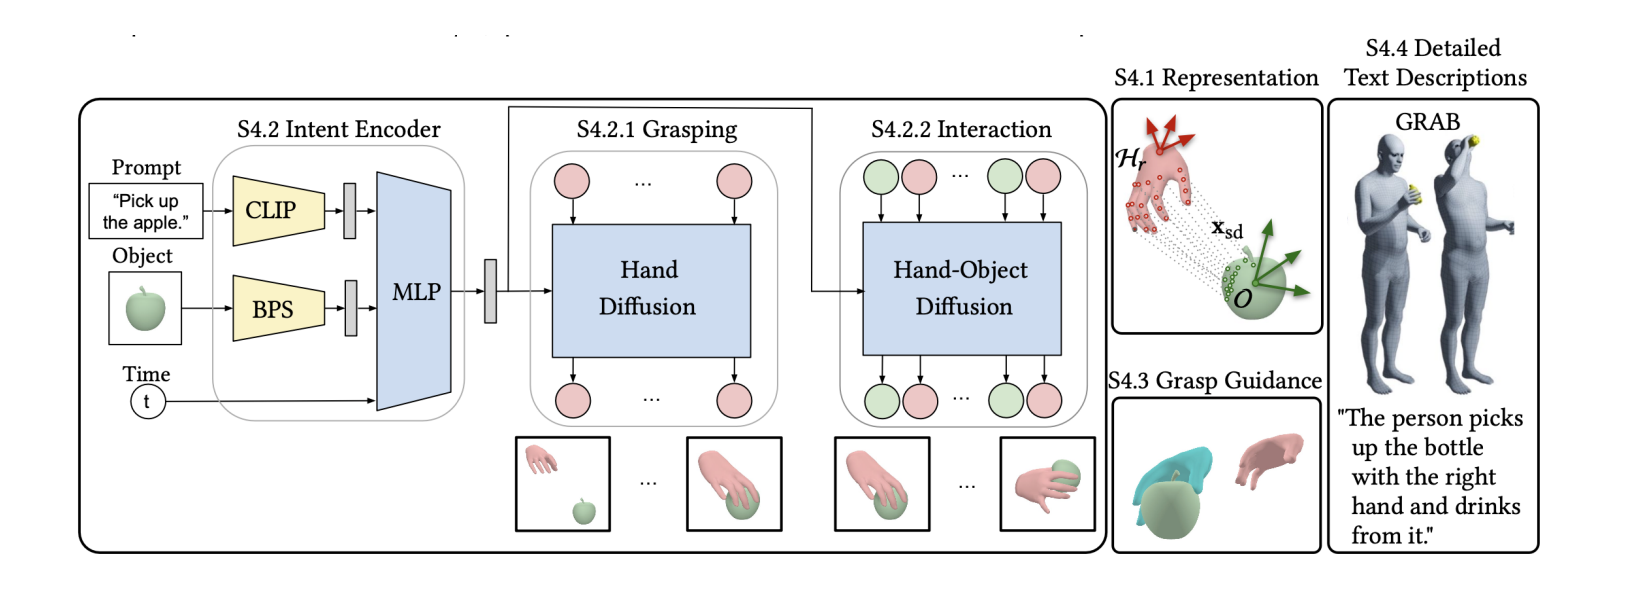
\includegraphics[width=\linewidth]{figure_2.png}
  \caption{\textbf{DiffH2O backbone (Segment Generator).} The Intent Encoder combines CLIP text embeddings with BPS object encodings. Phase~1 (Grasping) generates the hand approaching the object using a hand-only UNet denoiser with AdaGN conditioning. Phase~2 (Interaction) generates the full hand-object motion with the grasp inpainted as context. Our framework uses this backbone to generate each per-sentence segment.}
  \label{fig:diffh2o}
\end{figure}


% ============================================================
% 3. METHOD
% ============================================================
\section{Method}
\label{sec:method}

Given a multi-sentence text prompt $P = \{s_1, s_2, \ldots, s_N\}$, our goal is to generate a temporally coherent hand-object motion sequence $\mathcal{M} = [\bm_1, \btau_{1 \rightarrow 2}, \bm_2, \btau_{2 \rightarrow 3}, \ldots, \bm_N]$, where each $\bm_i \in \mathbb{R}^{T_i \times D}$ is a motion segment corresponding to sentence $s_i$ and each $\btau_{i \rightarrow i{+}1} \in \mathbb{R}^{T_\tau \times D}$ is a transition connecting consecutive segments.
Our framework consists of three modules: the Text Orchestrator (\cref{sec:orchestrator}), the Segment Generator (\cref{sec:segment_gen}), and the Switch Scheduler (\cref{sec:switch_scheduler}).
The full pipeline and post-processing are described in \cref{sec:pipeline}.

\subsection{Problem Formulation and Motion Representation}
\label{sec:representation}

\paragraph{Motion representation.}
Each frame of the motion is represented as a vector $\bx \in \mathbb{R}^D$.
For the GRAB dataset~\cite{taheri2020grab}, $D = 117$ and includes:
left and right hand PCA pose coefficients ($30$D each, comprising 3D position + 6D orientation + 21 PCA components),
left and right hand-to-object signed distance fields ($21$D each, one per MANO~\cite{romero2022mano} joint), and
object pose ($9$D: 3D position + 6D rotation representation).
For the OakInk2 dataset~\cite{zhan2024oakink2}, $D = 398$ and additionally includes:
body root translation and rotation ($9$D),
21 body joint rotations ($126$D in 6D representation),
left and right hand quaternion representations ($67$D each), and
up to three object poses ($27$D total), enabling bimanual multi-object manipulation with full SMPL-X~\cite{pavlakos2019expressive} body context.

\paragraph{Object representation.}
Object geometry is encoded using Basis Point Sets (BPS)~\cite{prokudin2019efficient}, a fixed-size representation that encodes the distance from a set of basis points to the nearest point on the object surface.
This provides the model with shape-aware conditioning independent of mesh resolution.

\paragraph{Forward diffusion process.}
Following DDPM~\cite{ho2020denoising}, we define a forward process that gradually adds Gaussian noise to a clean motion $\bx_0$:
\begin{equation}
    q(\bx_t | \bx_0) = \mathcal{N}(\bx_t; \sqrt{\bar{\alpha}_t}\, \bx_0, (1 - \bar{\alpha}_t)\, \mathbf{I}),
    \label{eq:forward}
\end{equation}
where $\bar{\alpha}_t = \prod_{s=1}^{t} \alpha_s$ and $\alpha_t = 1 - \beta_t$ with noise schedule $\{\beta_t\}_{t=1}^{T}$.


\subsection{Per-Sentence Segment Generation (DiffH2O Backbone)}
\label{sec:segment_gen}

Each sentence $s_i$ is processed by the DiffH2O backbone~\cite{christen2024diffh2o} (\cref{fig:diffh2o}) through two phases.

\paragraph{Intent encoder.}
The text $s_i$ is encoded using a frozen CLIP~\cite{radford2021learning} text encoder to obtain a 512-dimensional embedding $\bz_\text{text}$.
The target object's BPS encoding $\bz_\text{obj} \in \mathbb{R}^{3072}$ is concatenated with $\bz_\text{text}$ and projected through an MLP to produce the intent conditioning vector:
\begin{equation}
    \bc = \text{MLP}([\bz_\text{text}; \bz_\text{obj}]).
    \label{eq:intent}
\end{equation}

\paragraph{Phase 1: Grasping.}
A UNet-based denoiser with AdaGN conditioning~\cite{dhariwal2021diffusion} generates the grasping motion $\bm_i^\text{grasp}$, modeling only the hand features as the hand approaches and contacts the object.
The denoiser $\epsilon_\theta^\text{grasp}$ predicts the clean motion:
\begin{equation}
    \hat{\bx}_0^\text{grasp} = \frac{1}{\sqrt{\bar{\alpha}_t}}\left(\bx_t - \sqrt{1 - \bar{\alpha}_t}\, \epsilon_\theta^\text{grasp}(\bx_t, t, \bc)\right).
    \label{eq:grasp_denoise}
\end{equation}

\paragraph{Phase 2: Interaction.}
The full hand-object motion $\bm_i$ is generated by a second denoiser $\epsilon_\theta^\text{int}$ that operates on the complete feature vector.
The generated grasp is inpainted~\cite{lugmayr2022repaint} into the initial frames as conditioning context, ensuring a natural transition from approach to manipulation:
\begin{equation}
    \hat{\bx}_0^\text{int} = \frac{1}{\sqrt{\bar{\alpha}_t}}\left(\bx_t - \sqrt{1 - \bar{\alpha}_t}\, \epsilon_\theta^\text{int}(\bx_t, t, \bc, \bm_i^\text{grasp})\right).
    \label{eq:int_denoise}
\end{equation}

\paragraph{Classifier-free guidance.}
During sampling, classifier-free guidance~\cite{ho2022classifier} steers generation toward the text condition with scale $w$:
\begin{equation}
    \hat{\epsilon}({\bx}_t, t, \bc) = (1 + w)\, \epsilon_\theta(\bx_t, t, \bc) - w\, \epsilon_\theta(\bx_t, t, \varnothing),
    \label{eq:cfg}
\end{equation}
where $\varnothing$ denotes the unconditional (null) condition, trained with mask probability $p_\text{mask} = 0.1$.


\subsection{Switch Scheduler}
\label{sec:switch_scheduler}

The Switch Scheduler is a boundary-conditioned diffusion model that generates transitions $\btau_{i \rightarrow i{+}1}$ between consecutive segments $\bm_i$ and $\bm_{i{+}1}$.
Unlike prior long-term motion methods that use simple interpolation or two-pass refinement, the Switch Scheduler learns the distribution of natural transitions conditioned on surrounding context.

\paragraph{Architecture.}
The Switch Scheduler (\cref{fig:switch_arch}) is a transformer-based denoiser parameterized as follows.
Given a noisy transition $\bx_t \in \mathbb{R}^{T_\tau \times D}$ (default $T_\tau = 20$ frames), the model takes three conditioning inputs:
\begin{itemize}
    \item \textbf{Boundary frames}: The last $k$ frames of $\bm_i$ and first $k$ frames of $\bm_{i{+}1}$ (default $k{=}5$) are flattened and encoded via an MLP boundary encoder:
    \begin{equation}
        \bz_\text{bnd} = \text{MLP}_\text{bnd}\left([\bm_i[-k{:}] \,\|\, \bm_{i{+}1}[{:}k]]\right) \in \mathbb{R}^{d},
        \label{eq:boundary_enc}
    \end{equation}
    where $d = 512$ is the latent dimension.
    \item \textbf{Text conditioning}: CLIP embeddings of both adjacent sentences are concatenated and projected:
    \begin{equation}
        \bz_\text{txt} = \text{MLP}_\text{txt}\left([\bz_\text{text}^{(i)} \,\|\, \bz_\text{text}^{(i{+}1)}]\right) \in \mathbb{R}^{d}.
        \label{eq:text_enc}
    \end{equation}
    \item \textbf{Timestep embedding}: Sinusoidal embedding of the diffusion timestep $t$, projected to $\mathbb{R}^d$.
\end{itemize}

The transition is processed as: (i)~linear projection of each frame to the latent dimension, (ii)~addition of timestep, boundary, and text embeddings, (iii)~sinusoidal positional encoding, (iv)~$L$ transformer encoder layers with multi-head self-attention, and (v)~linear projection back to motion dimension:
\begin{equation}
    \hat{\bx}_0^\tau = f_\text{out}\left(\text{Transformer}\left(f_\text{in}(\bx_t) + \bz_t + \bz_\text{bnd} + \bz_\text{txt}\right)\right),
    \label{eq:switch_forward}
\end{equation}
where $f_\text{in}: \mathbb{R}^D \to \mathbb{R}^d$ and $f_\text{out}: \mathbb{R}^d \to \mathbb{R}^D$ are learned linear projections.
The transformer uses $L{=}8$ layers, $H{=}8$ attention heads, feed-forward dimension $1024$, and GELU activation.

\paragraph{Blend weight prediction.}
To ensure smooth boundaries, the model includes a learned blend weight predictor:
\begin{equation}
    w_\text{blend} = \sigmoid\left(\text{MLP}_\text{blend}(h_{\text{mid}})\right),
    \label{eq:blend_weight}
\end{equation}
where $h_\text{mid}$ is the latent representation at the temporal midpoint of the transition.
During composition, the transition is blended with boundary frames using a sigmoid ramp:
\begin{equation}
    \beta(t) = w_\text{blend} \cdot \sigmoid\left(10 \cdot (t / T_\tau - 0.5)\right), \quad t \in [0, T_\tau].
    \label{eq:sigmoid_ramp}
\end{equation}

\paragraph{Training objective.}
The Switch Scheduler is trained with the standard diffusion denoising objective on ground-truth transitions extracted from training data:
\begin{equation}
    \mathcal{L}_\text{switch} = \mathbb{E}_{\bx_0, \epsilon, t}\left[\| \bx_0 - \hat{\bx}_0^\tau(\bx_t, t, \bz_\text{bnd}, \bz_\text{txt}) \|^2\right].
    \label{eq:switch_loss}
\end{equation}

\paragraph{Inference.}
At inference, the transition is initialized via linear interpolation between the last frame of $\bm_i$ and the first frame of $\bm_{i{+}1}$, noise is added according to the forward process, and the model iteratively denoises over $T_\text{diff} = 100$ steps with a cosine noise schedule.
The final transition is blended with boundary frames via \cref{eq:sigmoid_ramp}.

\paragraph{Lightweight variant.}
For faster inference, we also provide a lightweight Switch Scheduler with $L{=}4$ layers, $H{=}4$ heads, feed-forward dimension $512$, and no dropout.


% ============================================================
% FIGURE 3: Switch Scheduler Architecture
% ============================================================
\begin{figure}[t]
  \centering
  \fbox{\parbox{0.95\linewidth}{\centering\vspace{2em}\textbf{[Switch Scheduler Architecture Diagram]}\\\vspace{0.5em}
  \small
  Boundary Encoder: MLP over last $k$ frames of $\bm_i$ + first $k$ frames of $\bm_{i{+}1}$\\
  Text Encoder: MLP over concatenated CLIP embeddings\\
  Timestep Embedder: Sinusoidal + MLP projection\\
  $\downarrow$ Sum all embeddings with projected input frames $\downarrow$\\
  Positional Encoding $\rightarrow$ 8$\times$ Transformer Layers $\rightarrow$ Output Projection\\
  $\downarrow$\\
  Blend Weight Predictor: MLP + Sigmoid $\rightarrow$ Sigmoid-Ramp Blending
  \vspace{2em}}}
  \caption{\textbf{Switch Scheduler architecture.} The model conditions on boundary frames, text embeddings, and diffusion timestep. A transformer backbone denoises the transition, and a learned blend weight predictor produces smooth boundary blending via a sigmoid ramp.}
  \label{fig:switch_arch}
\end{figure}


\subsection{Text Orchestration Module}
\label{sec:orchestrator}

The Text Orchestrator transforms a multi-sentence prompt $P$ into a structured generation plan. It performs four functions:

\paragraph{Sentence decomposition.}
The input paragraph is split into individual sentences using the NLTK~\cite{bird2009natural} sentence tokenizer, with a minimum length filter ($\geq 5$ characters) to discard fragments.

\paragraph{Object extraction.}
For each sentence, the orchestrator identifies the target object by dictionary matching against a list of known objects (54 objects for GRAB, extended for OakInk2).
A regex fallback captures objects from verb-object patterns (\eg, ``picks up the \emph{mug}'').

\paragraph{Temporal marker detection.}
Sentences are classified into four temporal types based on keyword matching: \emph{sequential} (``then'', ``next'', ``after''), \emph{simultaneous} (``while'', ``during''), \emph{beginning} (``first'', ``initially''), and \emph{ending} (``finally'', ``lastly'').
These markers inform the ordering and overlap of segments.

\paragraph{Duration planning.}
Each segment is assigned a frame count based on keyword heuristics:
actions containing speed modifiers (\eg, ``quickly'' $\rightarrow 0.7\times$, ``slowly'' $\rightarrow 1.3\times$, ``examines'' $\rightarrow 1.2\times$ the default 100 frames) are adjusted accordingly, with results clamped to $[50, 200]$ frames.
This produces the generation plan $\mathcal{G} = \{(s_i, o_i, T_i, \text{type}_i)\}_{i=1}^N$.


\subsection{Full Pipeline and Post-Processing}
\label{sec:pipeline}

The complete generation procedure is summarized in \cref{alg:pipeline}.

\begin{algorithm}[t]
\caption{Switch~\&~Stitch: Long-Horizon Hand-Object Motion Generation}
\label{alg:pipeline}
\begin{algorithmic}[1]
\REQUIRE Multi-sentence prompt $P$, DiffH2O model $\epsilon_\theta$, Switch Scheduler $f_\text{switch}$
\ENSURE Long-horizon motion sequence $\mathcal{M}$
\STATE $\mathcal{G} \leftarrow \text{TextOrchestrator}(P)$ \hfill \COMMENT{Parse text, extract plan}
\STATE $\{\bm_i\}_{i=1}^{N} \leftarrow \emptyset$
\FOR{each $(s_i, o_i, T_i) \in \mathcal{G}$}
    \STATE $\bm_i \leftarrow \text{SegmentGenerator}(s_i, o_i, T_i, \epsilon_\theta)$ \hfill \COMMENT{DiffH2O two-phase generation}
\ENDFOR
\STATE $\{\btau_{i \rightarrow i+1}\}_{i=1}^{N-1} \leftarrow \emptyset$
\FOR{$i = 1$ to $N-1$}
    \STATE $\btau_{i \rightarrow i+1} \leftarrow f_\text{switch}(\bm_i, \bm_{i+1}, s_i, s_{i+1})$ \hfill \COMMENT{Switch Scheduler diffusion}
    \STATE $\btau_{i \rightarrow i+1} \leftarrow \text{Blend}(\btau_{i \rightarrow i+1}, \bm_i, \bm_{i+1})$ \hfill \COMMENT{Sigmoid-ramp blending}
\ENDFOR
\STATE $\mathcal{M} \leftarrow [\bm_1, \btau_{1 \rightarrow 2}, \bm_2, \ldots, \btau_{N{-}1 \rightarrow N}, \bm_N]$ \hfill \COMMENT{Concatenate}
\STATE $\mathcal{M} \leftarrow \text{SmoothVelocities}(\mathcal{M})$ \hfill \COMMENT{3-frame boundary averaging}
\RETURN $\mathcal{M}$
\end{algorithmic}
\end{algorithm}

\paragraph{Velocity smoothing.}
After concatenation, we apply a 3-frame averaging window at each segment-transition boundary to eliminate residual velocity discontinuities:
\begin{equation}
    \bx_j' = 0.25\, \bx_{j-1} + 0.5\, \bx_j + 0.25\, \bx_{j+1},
    \label{eq:smooth}
\end{equation}
for frames $j$ within a $\pm 3$-frame window around each boundary.

\paragraph{Blending methods.}
The framework supports three transition blending strategies: (i)~\emph{smooth} (default): sigmoid-ramp blending using learned weights (\cref{eq:sigmoid_ramp}), (ii)~\emph{linear}: linearly interpolated blending weights, and (iii)~\emph{cubic}: Hermite spline interpolation~\cite{de1978practical} that matches boundary velocities for $C^1$ continuity.


% ============================================================
% 4. EXPERIMENTS (Placeholder)
% ============================================================
\section{Experiments}
\label{sec:experiments}

\paragraph{Datasets.}
We evaluate on two datasets.
\textbf{GRAB}~\cite{taheri2020grab} contains whole-body grasping sequences with 51 objects and text annotations.
Motion is represented as $117$D vectors at 30 FPS.
\textbf{OakInk2}~\cite{zhan2024oakink2} provides bimanual manipulation sequences with $398$D features including full SMPL-X body, dual hand representations, and multi-object support.
For long-horizon evaluation, we construct multi-sentence prompts by concatenating 2--5 consecutive action descriptions from the test sets.

\paragraph{Baselines.}
We compare against: (i)~\emph{Naive concatenation}: independently generated segments concatenated without transitions; (ii)~\emph{Linear interpolation}: segments connected via linear interpolation over $T_\tau = 20$ frames; (iii)~\emph{Cubic interpolation}: Hermite spline transitions matching boundary velocities; (iv)~\emph{DoubleTake}~\cite{shafir2024doubletake} adapted for hand-object features; (v)~\emph{FlowMDM}~\cite{barquero2024seamless} adapted for hand-object features.

\paragraph{Metrics.}
We evaluate using: (i)~\emph{FID}~\cite{heusel2017gans} on per-segment motion quality; (ii)~\emph{Transition smoothness}: average jerk (third derivative) at segment boundaries; (iii)~\emph{Contact consistency}: percentage of frames with valid hand-object contact during transitions; (iv)~\emph{Object position error}: L2 distance between object pose at segment end and next segment start; (v)~\emph{Text-motion alignment}: CLIP-based similarity between generated motion and input text.

\paragraph{Quantitative results.}
\cref{tab:results} presents placeholder results.
Full experimental results will be included upon completion of the evaluation pipeline.

\begin{table}[t]
  \caption{Quantitative comparison on GRAB dataset (placeholder values). $\downarrow$~indicates lower is better, $\uparrow$~indicates higher is better. Best results in \textbf{bold}.}
  \label{tab:results}
  \centering
  \begin{tabular}{@{}lccccc@{}}
    \toprule
    Method & FID $\downarrow$ & Jerk $\downarrow$ & Contact $\uparrow$ & Obj. Err. $\downarrow$ & Text Sim. $\uparrow$ \\
    \midrule
    Naive concat.    & -- & -- & -- & -- & -- \\
    Linear interp.   & -- & -- & -- & -- & -- \\
    Cubic interp.    & -- & -- & -- & -- & -- \\
    DoubleTake~\cite{shafir2024doubletake} & -- & -- & -- & -- & -- \\
    FlowMDM~\cite{barquero2024seamless}   & -- & -- & -- & -- & -- \\
    \midrule
    \textbf{Ours}    & -- & -- & -- & -- & -- \\
    Ours (lightweight) & -- & -- & -- & -- & -- \\
    \bottomrule
  \end{tabular}
\end{table}


% ============================================================
% 5. CONCLUSION
% ============================================================
\section{Conclusion}
\label{sec:conclusion}

We presented Switch~\&~Stitch, the first framework for generating long-horizon hand-object manipulation sequences from multi-sentence natural language descriptions.
Our approach combines a Text Orchestrator for structured prompt decomposition, the DiffH2O backbone for per-sentence segment generation, and a novel Switch Scheduler---a boundary-conditioned diffusion transformer---for generating smooth, physically plausible transitions between segments.
We demonstrated the framework on the GRAB and OakInk2 datasets, showing that learned transitions outperform interpolation baselines in terms of motion smoothness, contact consistency, and temporal coherence.
Future work includes training the Switch Scheduler end-to-end with the segment generator, extending to simultaneous bimanual manipulation, and incorporating physics-based contact refinement.


% ---- Bibliography ----
\bibliographystyle{splncs04}
\bibliography{main}
\end{document}
